\section{218 --- The Skyline Problem}
A city's skyline is the outer contour of the silhouette formed by all the buildings in that city when viewed from a distance. Now suppose you are given \textbf{the locations and height of all the buildings} as shown on a cityscape photo (Figure A), write a program to \textbf{output the skyline} formed by these buildings collectively (Figure B).
\renewcommand{\thesubfigure}{\Alph{subfigure}}
\begin{figure}[H]
\begin{subfigure}[b]{8cm}
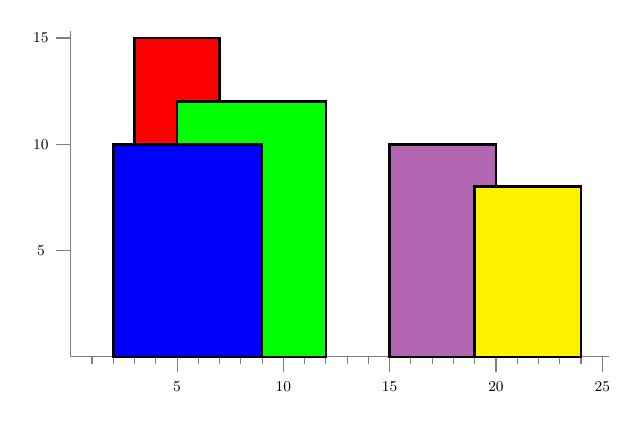
\begin{tikzpicture}[scale=0.9,every node/.style={scale=0.6}]
\draw[color=black!50!] (0,0) -- (7.6,0);
\draw[color=black!50!] (0,0) -- (0, 4.6);
\foreach \x in {0.3,0.6,...,7.5}
\draw[color=black!50!] (\x, -3pt) -- (\x, 0);
\foreach \x in {5,10,...,25}
{
\draw[color=black!50!] (\x*0.3, -6pt) -- (\x*0.3, 0);
\node at (\x*0.3,-12pt) {\small \x};
}
\foreach \y in {5,10,...,15}
{
\draw[color=black!50!] (-6pt,\y*0.3) -- (0, \y*0.3);
\node at (-12pt, \y*0.3) {\small \y};
}
\filldraw[draw=black, line width=1pt, fill=red] (0.9, 0) rectangle (2.1,4.5);
\filldraw[draw=black, line width=1pt, fill=green] (1.5,0) rectangle (3.6,3.6);
\filldraw[draw=black, line width=1pt, fill=blue] (0.6, 0) rectangle (2.7,3.0);
\filldraw[draw=black, line width=1pt, fill=violet!60!white] (4.5, 0) rectangle (6,3);
\filldraw[draw=black, line width=1pt, fill=yellow] (5.7, 0) rectangle (7.2,2.4);
\end{tikzpicture}
\caption{Buildings}
\end{subfigure}
\begin{subfigure}[b]{8cm}
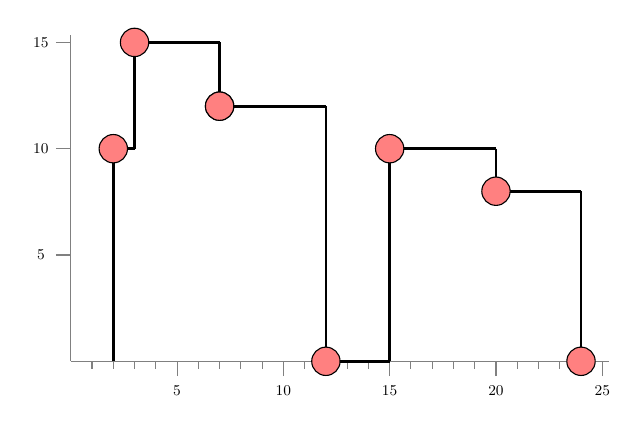
\begin{tikzpicture}[scale=0.9,every node/.style={scale=0.6}]
\draw[color=black!50!] (0,0) -- (7.6,0);
\draw[color=black!50!] (0,0) -- (0, 4.6);
\foreach \x in {0.3,0.6,...,7.5}
\draw[color=black!50!] (\x, -3pt) -- (\x, 0);
\foreach \x in {5,10,...,25}
{
\draw[color=black!50!] (\x*0.3, -6pt) -- (\x*0.3, 0);
\node at (\x*0.3,-12pt) {\small \x};
}
\foreach \y in {5,10,...,15}
{
\draw[color=black!50!] (-6pt,\y*0.3) -- (0, \y*0.3);
\node at (-12pt, \y*0.3) {\small \y};
}
\draw[line width=1pt] (0.6,0) -- (0.6,3);

\draw[line width=1pt] (0.6,3) -- (0.9,3);
\draw[line width=1pt] (0.9,3) -- (0.9,4.5);

\draw[line width=1pt] (0.9,4.5) -- (2.1,4.5);
\draw[line width=1pt] (2.1,4.5) -- (2.1,3.6);
\draw[line width=1pt] (2.1,3.6) -- (3.6,3.6);
\draw[line width=1pt] (3.6,3.6) -- (3.6, 0);
\draw[line width=1pt] (3.6,0) -- (4.5, 0);
\draw[line width=1pt] (4.5,0) -- (4.5, 3);
\draw[line width=1pt] (4.5,3) -- (6,3);
\draw[line width=1pt] (6,3) -- (6, 2.4);
\draw[line width=1pt] (6,2.4) -- (7.2, 2.4);
\draw[line width=1pt] (7.2,2.4) -- (7.2, 0);

\draw[fill=red!50!] (0.6,3) circle (2mm);
\draw[fill=red!50!] (0.9,4.5) circle (2mm);
\draw[fill=red!50!] (2.1,3.6) circle (2mm);
\draw[fill=red!50!] (3.6,0) circle (2mm);
\draw[fill=red!50!] (4.5,3) circle (2mm);
\draw[fill=red!50!] (2.1,3.6) circle (2mm);
\draw[fill=red!50!] (6,2.4) circle (2mm);
\draw[fill=red!50!] (7.2,0) circle (2mm);
\end{tikzpicture}
\caption{Silhouettes}
\end{subfigure}
\end{figure}
The geometric information of each building is represented by a triplet of integers $[L_i, R_i, H_i]$, where $L_i$ and $R_i$ are the $x$ coordinates of the left and right edge of the $i$th building, respectively, and $H_i$ is its height. It is guaranteed that $0 \leq L_i, R_i \leq$ \texttt{INT\_MAX}, $0 < H_i \leq$ \texttt{INT\_MAX}, and $R_i - L_i > 0$. You may assume all buildings are perfect rectangles grounded on an absolutely flat surface at height 0.
\par
For instance, the dimensions of all buildings in Figure A are recorded as:
$[2, 9, 10]$, $[3, 7, 15]$, $[5, 12, 12]$, $[15, 20, 10]$, $[19, 24, 8]$.
\par
The output is a list of \textit{key points} (red dots in Figure B) in the format of $[x_1,y_1]$, $[x_2, y_2]$, $[x_3, y_3]$, $\ldots$ that uniquely defines a skyline. A \textit{key point} is the left endpoint of a horizontal line segment. Note that the last key point, where the rightmost building ends, is merely used to mark the termination of the skyline, and always has zero height. Also, the ground in between any two adjacent buildings should be considered part of the skyline contour.
\par
For instance, the skyline in Figure B should be represented as:
$
[2, 10]$, $[3, 15]$, $[7, 12]$, $[12, 0]$, $[15 ,10]$, $[20, 8]$, $[24, 0]$

\paragraph{Notes:}
\begin{itemize}
    \item The number of buildings in any input list is guaranteed to be in the range $[0, 10000].$
    \item     The input list is already sorted in ascending order by the left $x$ position $L_i$.
    \item The output list must be sorted by the $x$ position.
    \item There must be no consecutive horizontal lines of equal height in the output skyline. For instance, $[2, 3]$, $[4, 5]$, $[7, 5]$, $[11, 5]$, $[12, 7]$ is not acceptable; the three lines of height 5 should be merged into one in the final output as such: $[2, 3], [4, 5], [12, 7]$
\end{itemize}
\subsection{Sorting}
\begin{itemize}
    \item 每个矩形的左上角和右上角是可能的轮廓变化点,称之为critical points。
    \item 如果相邻的两个矩形不重叠,左边矩形的右下角也是key point。
    \item 如果某个critical point处在一个矩形的左右边的范围内(即比较$x$坐标),那么这个轮廓变化点处的高度为这个点之前的高度和当前矩形的高度的最大值。
    \item 为了快速得到所有包含某个critical point的矩形高度的最大值,可以用一个maximum heap来进行排序。
\end{itemize}
算法大致过程如下:
\begin{enumerate}
    \item sort all the critical points. 
    \item 从左到右扫描上述排序后的critical points。如果遇到某个矩形的左边,就将这个矩形加入到heap中。如果遇到某个矩形的右边,就将这个矩形从heap中remove。
    \item 记录当前的最大高度,以及上一次的最大高度,如果发生改变,表示遇到了一个key point了。
    \item 最后,每次遇到critical point,将其高度更新为当前heap的top,即当前在heap中的所有矩形的高度的最大值。
\end{enumerate}
几个coding的技巧
\begin{itemize}
    \item 可以将矩形左边界的高度设置为负数,这样就很容易区分当前遇到的是矩形的左边界还是右边界了。
    \item 用\texttt{multiset}作为存放矩形高度的数据结构,因为\texttt{priority queue}不提供删除操作。
    \item 在遍历critical points之前,将0放入到heap中,因为最后的矩形的右下角总是要包含在key point中的。
\end{itemize}
\setcounter{algorithm}{0}
\begin{algorithm}[H]
\caption{Heap Based Sorting}
\begin{algorithmic}[1]
\Procedure{GetSkyline}{$B, L$}
\State $\star$ sort all left and right points in $B$
\State $H_0:=0$ \Comment Last maximum height
\For{Each sorted point $p$}
\If{$p$ is the left edge of a rectangle}
\State $\star$ Add $p$ to the heap
\Else
\State $\star$ Remove $p$ from the heap
\EndIf
\State $\star$ Get current maixmum height $H$ from the heap
\If{$H_0\neq H$} \Comment A key point is found
\State $\star$ Add $p$'s $x$ coordinate and $H$ into the result array
\State $H_0\gets H$ \Comment Update last maximum height
\EndIf
\EndFor
\State $\star$ Returns the result array
\EndProcedure
\end{algorithmic}
\end{algorithm}
\setcounter{lstlisting}{0}
\begin{lstlisting}[style=customc, caption={Sorting}]
public:
vector<pair<int, int>> getSkyline( vector<vector<int>>& buildings )
{

    set<pair<int, int>> pt_sets;

    for( const auto& b : buildings )
    {
        pt_sets.emplace( b[0], -b[2] );
        pt_sets.emplace( b[1], b[2] );
    }

    multiset<int> h_sets;
    h_sets.insert( 0 );

    int pre_h = 0;
    int cur_h = 0;

    vector<pair<int, int>> ans;

    for( const auto&pt : pt_sets )
    {
        if( pt.second < 0 )
        {
            h_sets.insert( -pt.second );
        }
        else
        {
            // h_sets.erase(pt.second) will remove all 
            // keys that equal to pt.second. It is not desired
            // since we want to remove only one element.
            h_sets.erase( h_sets.find( pt.second ) );
        }

        cur_h = *( h_sets.rbegin() );

        if( cur_h != pre_h )
        {
            ans.emplace_back( pt.first, cur_h );
            pre_h = cur_h;
        }
    }

    return ans;
}

\end{lstlisting}
